\subsection{\href{\linknovo}{NOVO SPACE}}
   \hypertarget{subsec:novo_space}
   I worked for a year at an exciting aerospace start-up as an embedded systems leader. I've developed firmware for complex SoCs, analysis of new technologies, port of bootloaders, port of embedded linux, device drivers, baremetal C and ASM startup coding, analysis of aerospace software, among other related activities. I've worked in a team with other 15 specialists, but I quit due to moving to another country.

     \begin{figure}
      \begin{center}
         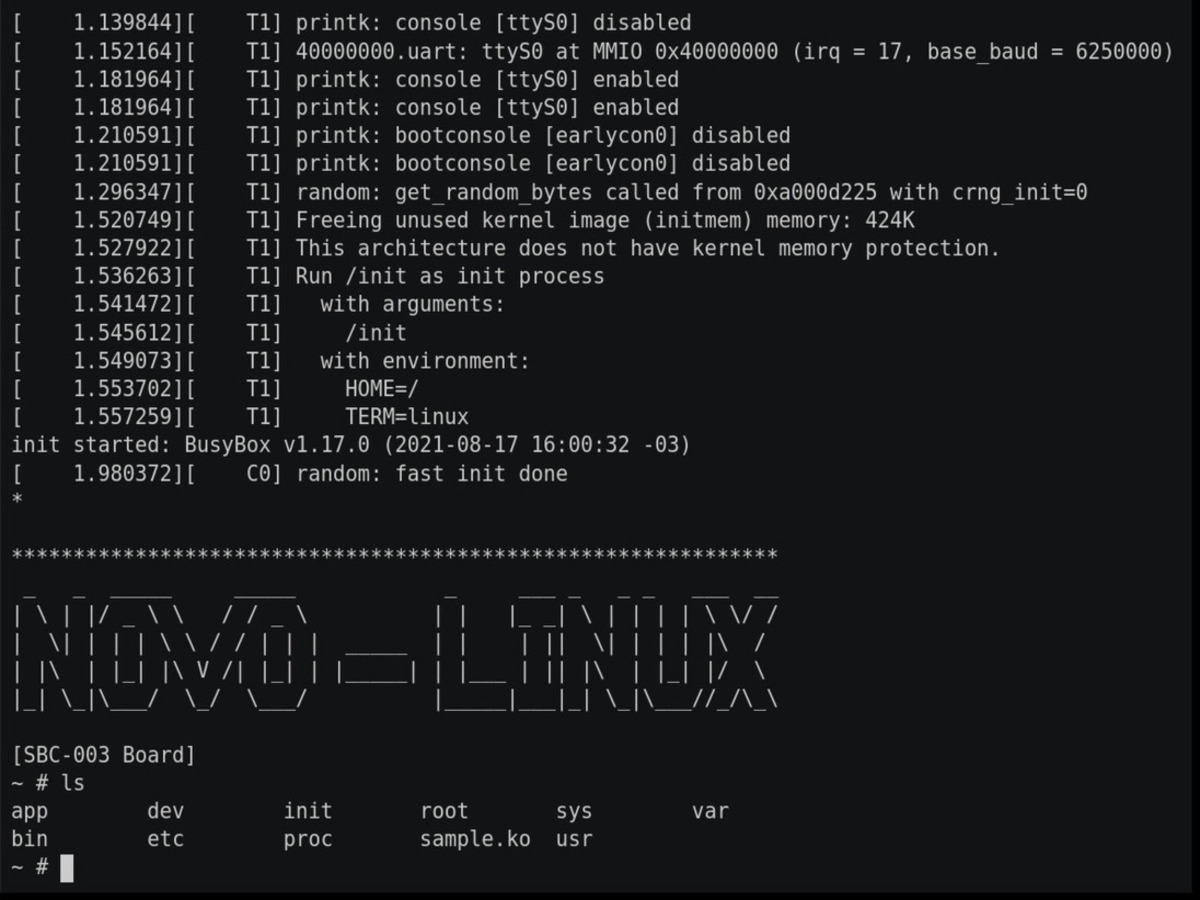
\includegraphics[width=0.3\textwidth]{novo1.jpg}
         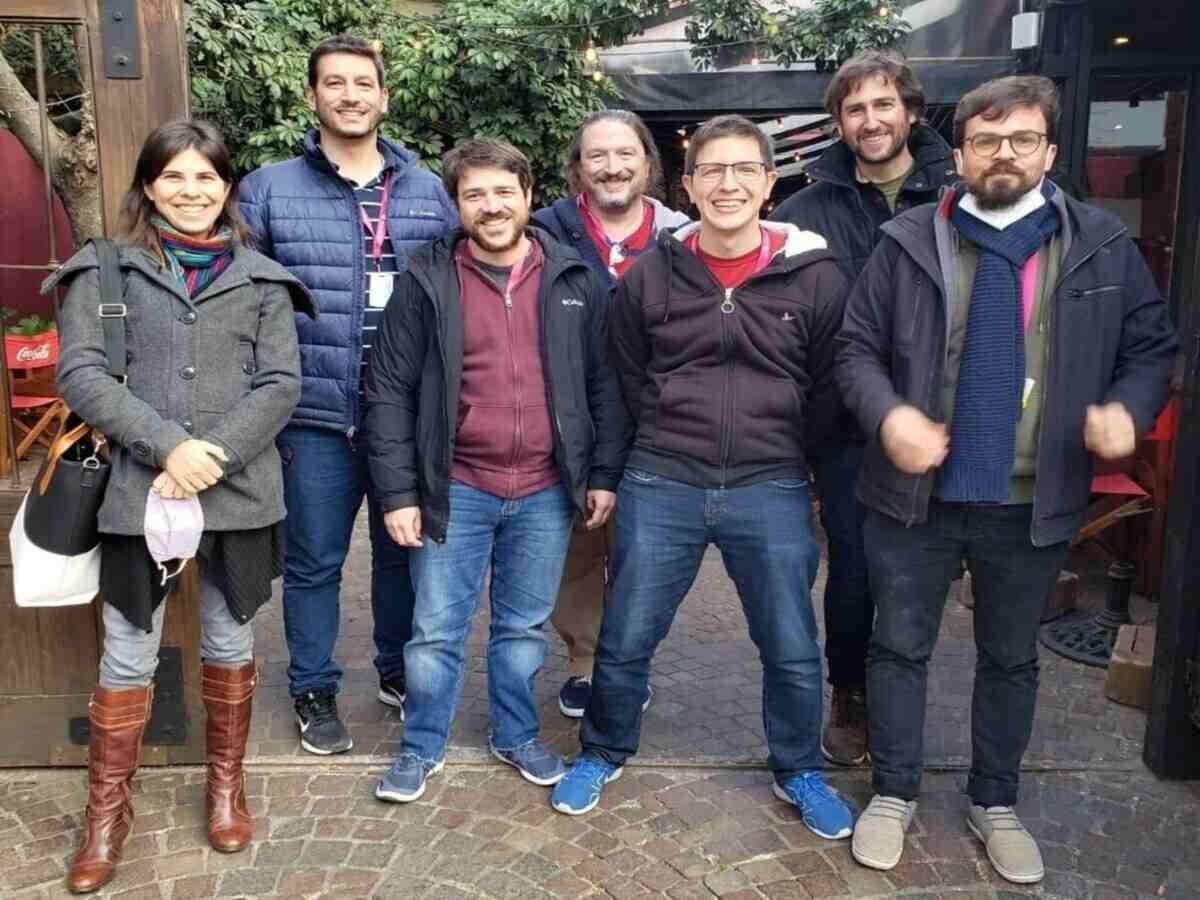
\includegraphics[width=0.3\textwidth]{novo3.jpg}
         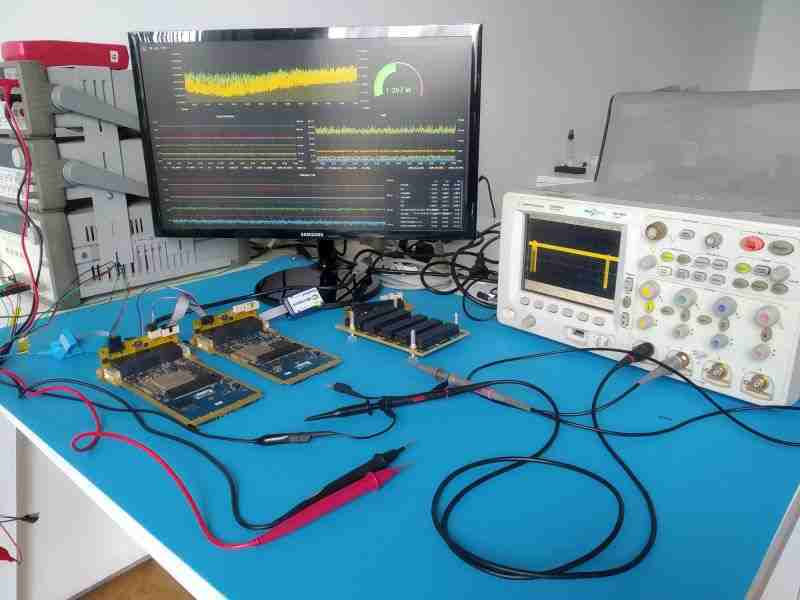
\includegraphics[width=0.3\textwidth]{novo4.jpg}
      \end{center}
        \caption{A capture of an embedded Linux (left) ported from scratch and running on NOVO SPACE boards (right).}
      \label{fig:novo_space}
   \end{figure}

%---------------------------------------------------
\ifdefined\portfolioFull
During my job at \href{\linknovo}{NOVO SPACE} I mainly work as a lead firmware developer.
At the begining the main focus of the job was:
      \cvlistitem{Bringup the fresh new NOVO boards}
      \cvlistitem{Write startup firmware for SoC's (ARM C-M0 with FPGA)}
      \cvlistitem{Write FPGA interfaces and connect them with firmware drivers}
      \cvlistitem{Golden mode firmware image recover}
      \cvlistitem{Reliance edge, wear leveling capable file system port/choose/select/implement}
      \cvlistitem{Memory stress test}
      \cvlistitem{Telemetry report of main internal values from the very early code until main app runs}
      \cvlistitem{Bootloader develop/port}
      \cvlistitem{u-boot as a general bootloader ported to a very constrained M0 and without DDR}
      \cvlistitem{FreeRtos ported to M0, DDR access through FPGA and then a file system over that was mounted.}
      \cvlistitem{NASA CFS ground app connected with the boards}
      \cvlistitem{DAP protocol access from python script to a memory mapped internal bank as a telemetry}
      \cvlistitem{Port and run custom \textless800kB Linux kernel + FS for C-M0, with custom timer and UART device drivers with a minimal busybox RAM file system and launched from a custom u-boot from NOR to DDR.} 
      \cvlistitem{HUGO documentation and gitlab CI/CD daily use.} 
     \begin{figure}
      \begin{center}
         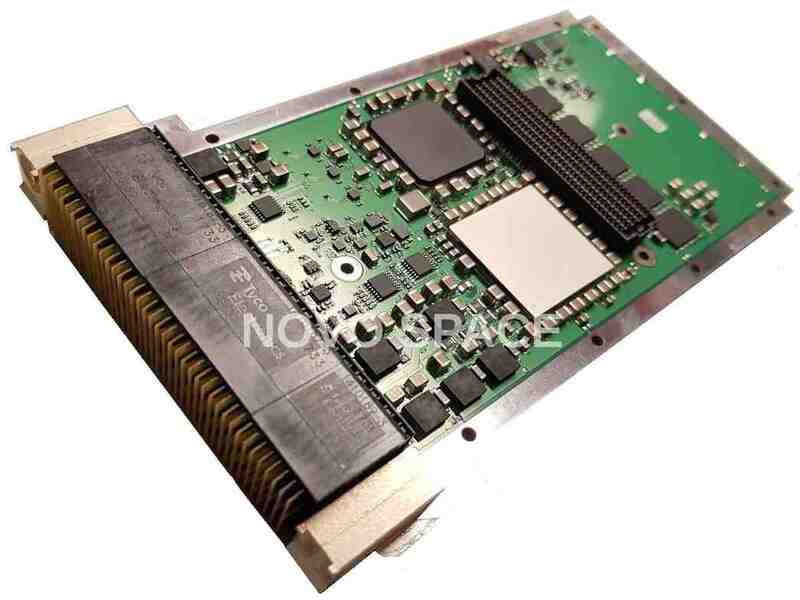
\includegraphics[width=0.3\textwidth]{novo5.jpg}
         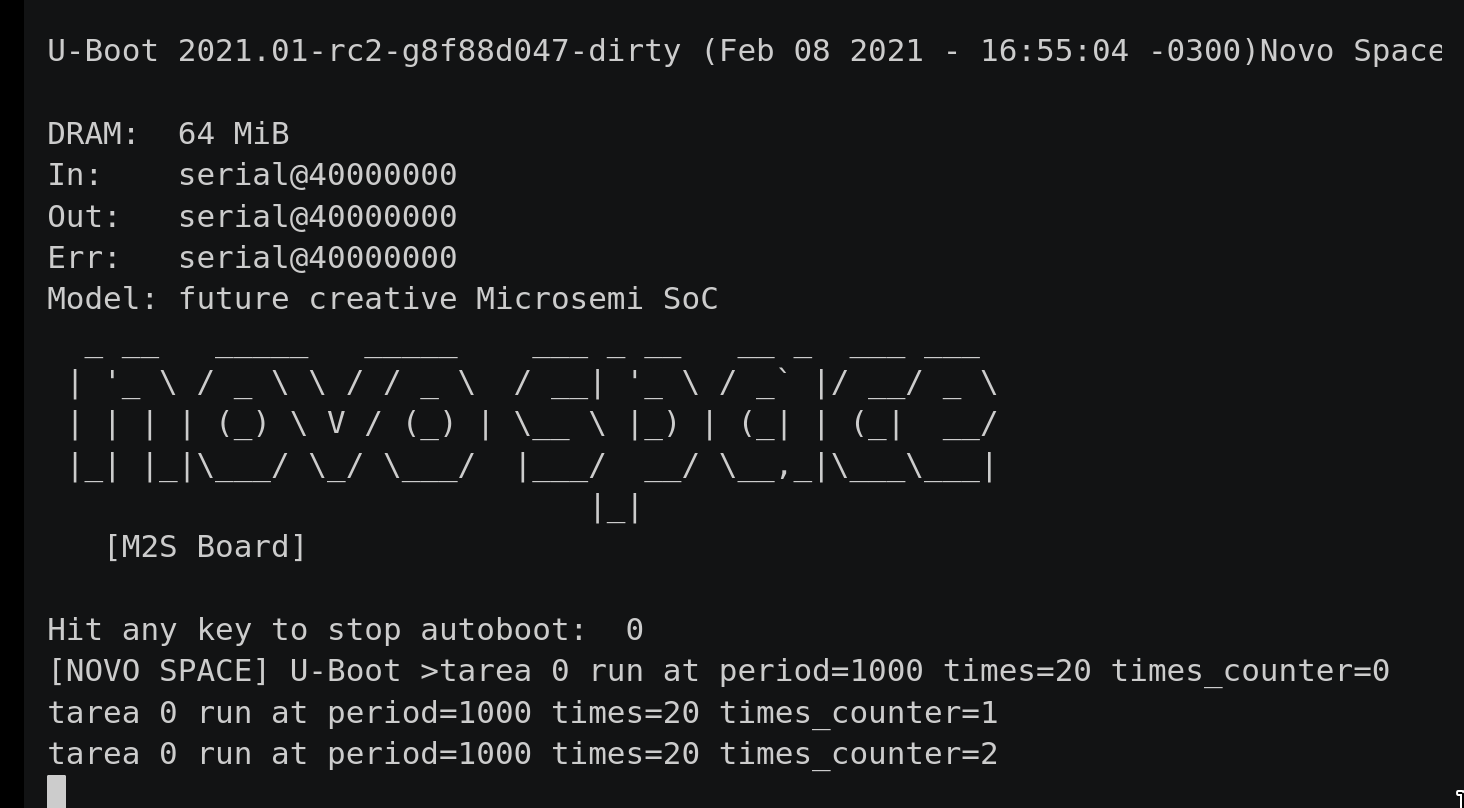
\includegraphics[width=0.3\textwidth]{novo6.jpg}
         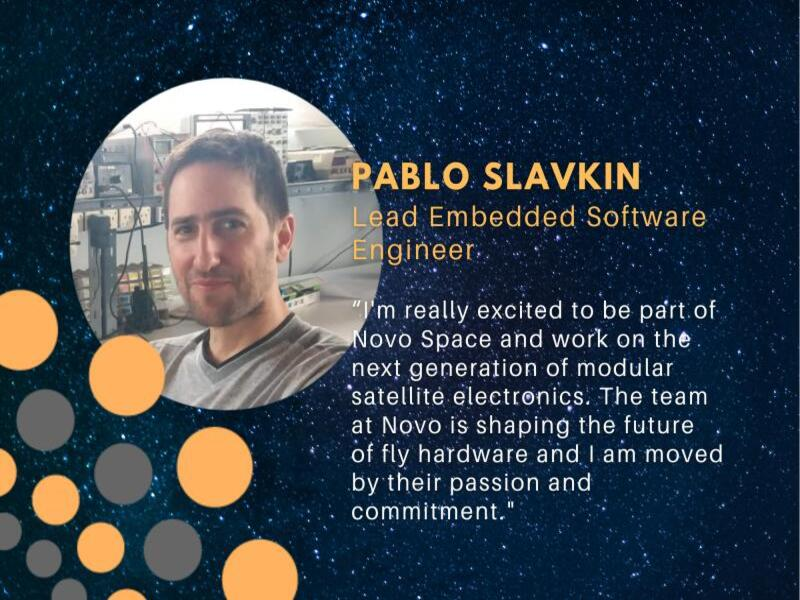
\includegraphics[width=0.3\textwidth]{novo7.jpg}
      \end{center}
        \caption{Novo super high speed and complex boards with a u-boot running on it.}
      \label{fig:novo_space}
   \end{figure}
\pagebreak
%---------------------------------------------------
\fi

